\chapter{开始}
\subsection{开始TensorFlow}
这个向导,你将开始使用TensorFlow编程。在开始本文之前,\href{https://www.tensorflow.org/install/index}{安装TensorFlow}。为了理解这个向导,你将需要:
\begin{itemize}
\item 如何使用Python编程
\item 了解一点数组
\item 了解机器学习更好。即使,你不太了解机器学习,这篇文章仍然应该是你的第一个向导。
\end{itemize}
TensorFlow提供了多个API。最低的TensorFlow 核心API提供给你完整的程序控制。更高级的API构建在TensorFlow核心之上。这些高级API通常比TensorFlow核心更容易阅读和使用。另外,更高级的API使得用户之间重复的任务变得更容易。一像tf.estimator的高级API帮助你管理数据集,estimators,训练和推理。

这个向导以TensorFlow核心开始。之后,我们展示如何在tf.estimators中实现相同的模型。了解TensorFlow核心规则将在你使用更复杂的高级API时给你一个内部工作的思维模型。
\subsection{Tensors}
TensorFlow中数据的核心单元是tensor。一个tensor组成了任意维度数据的值。一个tensor的rank是他的维数。这里有一些例子:
\begin{pythoncode}
# a rank 0 tensor; a scalar with shape []
[1., 2., 3.] # a rank 1 tensor; a vector with shape [3]
[[1., 2., 3.], [4., 5., 6.]] # a rank 2 tensor; a matrix with shape [2, 3]
[[[1., 2., 3.]], [[7., 8., 9.]]] # a rank 3 tensor with shape [2, 1, 3]
\end{pythoncode}
\subsection{TensorFlow核心导航}
\subsubsection{导入TensorFlow}
规范的TensorFlow程序导入如下:
\begin{pythoncode}
import tensorflor as tf 
\end{pythoncode}
这让Python能访问TensorFlow的任何类,方法,符号。多数文档假设你已经有了这。
\subsubsection{计算图}
你也许可以考虑TensorFlow核心程序为下面的两个部分:
\begin{itemize}
\item 构建计算图
\item 运行计算图
\end{itemize}
一个计算图是一系列的安排在图上节点的TensorFlow操作。让我们构建一个简单的计算图,每个节点接收0或者更多的tensor作为输入产生一个tensor作为输出。一个典型的节点是常数。像所有的TensorFlow常数,它不接收输入,输出一个存储在其内部的值。我们可以创建两个浮点Tensor node1和node2:

\begin{pythoncode}
node1 = tf.constant(3.0, dtype=tf.float32)
node2 = tf.constant(4.0) # also tf.float32 implicitly
print(node1, node2)
\end{pythoncode}

最终生成打印:
\begin{pythoncode}
Tensor("Const:0", shape=(), dtype=float32) Tensor("Const_1:0", shape=(), dtype=float32)
\end{pythoncode}
注意打印节点不像你想的那样输出值3.0和4.0,而是他们是节点,当计算时对应的产生3.0和4.0。为了计算节点,你必须用session运行计算图。一个会话是TensorFlow控制和运行环境的集合体。

下面的代码创建一个Session对象,然后调用run方法运行计算图计算node1和node2.默认会话中的计算图如下:
\begin{pythoncode}
sess = tf.Session()
print(sess.run([node1, node2]))
\end{pythoncode}
我们将看到我们想要的输出3.0和4.0:
\begin{pythoncode}
[3.0,4.0]
\end{pythoncode}
你可以通过结合Tensor节点和操作构建更复杂的计算。例如,你可以添加两个常数节点生成一个新的图:
\begin{pythoncode}
from __future__ import print_function
node3 = tf.add(node1, node2)
print("node3:", node3)
print("sess.run(node3):", sess.run(node3))
\end{pythoncode}
最后的打印声明产生:
\begin{pythoncode}
node3: Tensor("Add:0", shape=(), dtype=float32)
sess.run(node3): 7.0
\end{pythoncode}
TensorFlow提供一个称为TensorBoard的实用程序,你可以显示一个计算图。这里的截图显示了TensorBoard如何可视化图:
\begin{figure}[H]
\centering
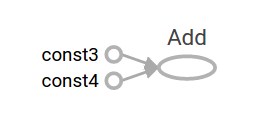
\includegraphics{getting_started_add.png}
\caption{计算图}
\end{figure}
正如上面表示,图并不特别有趣因为它总是产生一个常数结果。一个图可以参数化接收内部输入正如placeholders。一个placeholder
\begin{pythoncode}
a = tf.placeholder(tf.float32)
b = tf.placeholder(tf.float32)
adder_node = a + b  # + provides a shortcut for tf.add(a, b)
\end{pythoncode}
上面的三行代码像一个函数或者lambda表达式,我们定义了两个输入参数(a,b)和一个在他们之上的操作。我们可以通过feed\_dict参数结合多输入计算这个图用\href{https://www.tensorflow.org/api_docs/python/tf/Session#run}{run方法}输入具体的值给placeholders:
\begin{pythoncode}
print(sess.run(adder_node, {a: 3, b: 4.5}))
print(sess.run(adder_node, {a: [1, 3], b: [2, 4]}))
\end{pythoncode}
输出结果:
\begin{pythoncode}
7.5
[ 3.  7.]
\end{pythoncode}
在TensorBoard中图看起来像这样:
\begin{figure}[H]
\centering
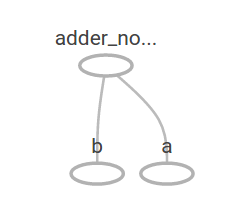
\includegraphics{getting_started_adder.png}
\caption{placeholder}
\end{figure}
你可以通过添加一个另一个操作使得计算图更复杂。例如:
\begin{pythoncode}
add_and_triple = adder_node * 3.
print(sess.run(add_and_triple, {a: 3, b: 4.5}))
\end{pythoncode}
产生输出:22.5。
上面的计算图在TensorBoard中像这样:
\begin{figure}[H]
\centering
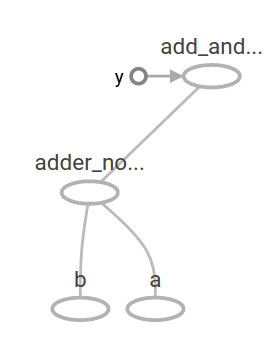
\includegraphics[scale=0.5]{getting_started_triple.png}
\caption{添加操作}
\end{figure}
在机器学习中我们通常接收任意输入,正如上面。为了使得模型可训练,我们需要能修改图获取相同输入的新的输出。Variable允许我们添加可训练的参数到图上。他们通过类型和初始值构造:
\begin{pythoncode}
W = tf.Variable([.3], dtype=tf.float32)
b = tf.Variable([-.3], dtype=tf.float32)
x = tf.placeholder(tf.float32)
linear_model = W*x + b
\end{pythoncode}
当你调用tf.constant时常数被初始化,他们的值不能改改。对比之下,当你调用tf.Variable的时候变量没有被初始化。为了初始化在TensorFlow程序中的所有变量,你必须明确的调用一个像下面的类似操作:
\begin{pythoncode}
init = tf.global_variables_initializer()
sess.run(init)
\end{pythoncode}
实现init处理TensorFlow子图初始化所有变量是很重要的。直到我们调用sess.run,变量才被初始化。
因为x是一个placeholder,我们可以按照下面同时通过多个x计算多个linear\_model:
\begin{pythoncode}
print(sess.run(linear_model, {x: [1, 2, 3, 4]}))
\end{pythoncode}
为了产生输出:
\begin{pythoncode}
[ 0.          0.30000001  0.60000002  0.90000004]
\end{pythoncode}
我们已经创建了一个模型,但是我们不知道它有多么好。为了在训练集上估计模型,我们需要一个placeholder提供想要的值,并且我们需要一个损失函数。

一个损失函数从提供的数据计算模型效果。我们将用标准的线性回归损失函数计算当前模型和提供数据之间的均方差。linear\_model -y创建一个向量,向量的每一个元素是对应的样本的误差。我们可以调用tf.square计算误差的平方,然后我们使用tf.reduce\_sum对所有的误差求和创建一个标量:
\begin{pythoncode}
y = tf.placeholder(tf.float32)
squared_deltas = tf.square(linear_model - y)
loss = tf.reduce_sum(squared_deltas)
print(sess.run(loss, {x: [1, 2, 3, 4], y: [0, -1, -2, -3]}))
\end{pythoncode}
产生损失值23.66。

我们可以通过手动赋值W,h为-1,1做出改变。一个变量被初始化值提供给tf.Variable但是可以使用想tf.assign这样的操作改变。例如,W=-1,和b=1对我们的模型来说是最优的参数。我们可以改变W和b:
\begin{pythoncode}
fixW = tf.assign(W, [-1.])
fixb = tf.assign(b, [1.])
sess.run([fixW, fixb])
print(sess.run(loss, {x: [1, 2, 3, 4], y: [0, -1, -2, -3]}))
\end{pythoncode}
最后的打印结果显示损失现在为0.0。

我们猜测W和b的最佳值,但是机器学习的最终目的是自动找到正确的模型参数。我们将在下面的章节显示如何完成。

\subsubsection{tf.train API}
为了完成这个导航的机器学习讨论。然而,TensorFlow提供优化器通过损失对变量的微分慢慢改变变量的值。通常,手动计算符号微分是很可笑的并且易出错。因此TensorFlow可以使用tf.gradients自动的生成给定描述的模型的微分。简单起见,优化器通常已经为你做好。例如:
\begin{pythoncode}
optimizer = tf.train.GradientDescentOptimizer(0.01)
train = optimizer.minimize(loss)
sess.run(init) # reset values to incorrect defaults.
for i in range(1000):
  sess.run(train, {x: [1, 2, 3, 4], y: [0, -1, -2, -3]})
print(sess.run([W, b]))
\end{pythoncode}
最终模型的参数:
\begin{pythoncode}
[array([-0.9999969], dtype=float32), array([ 0.99999082], dtype=float32)]
\end{pythoncode}
现在我们已经做了实际上的机器学习。尽管这个简单的线性回归模型不要求更多的TensorFlow核心代码,更复杂的输入数据到你的模型的方法需要更多代码。这样TensorFlow提供更高级的的常用样例,结构,功能抽象。我们将在下面的章节学习如何使用这些抽象。
\subsubsection{完整的代码}
完整的训练线性回归模型的代码:
\begin{pythoncode}
import tensorflow as tf

# Model parameters
W = tf.Variable([.3], dtype=tf.float32)
b = tf.Variable([-.3], dtype=tf.float32)
# Model input and output
x = tf.placeholder(tf.float32)
linear_model = W*x + b
y = tf.placeholder(tf.float32)

# loss
loss = tf.reduce_sum(tf.square(linear_model - y)) # sum of the squares
# optimizer
optimizer = tf.train.GradientDescentOptimizer(0.01)
train = optimizer.minimize(loss)

# training data
x_train = [1, 2, 3, 4]
y_train = [0, -1, -2, -3]
# training loop
init = tf.global_variables_initializer()
sess = tf.Session()
sess.run(init) # reset values to wrong
for i in range(1000):
  sess.run(train, {x: x_train, y: y_train})

# evaluate training accuracy
curr_W, curr_b, curr_loss = sess.run([W, b, loss], {x: x_train, y: y_train})
print("W: %s b: %s loss: %s"%(curr_W, curr_b, curr_loss))
\end{pythoncode}
运行产生:
\begin{pythoncode}
W: [-0.9999969] b: [ 0.99999082] loss: 5.69997e-11
\end{pythoncode}
注意损失很小(非常接近于0).如果你运行这个代码,你的损失也许不和上面的损失一样,这是因为模型实用伪随机数值初始化。

更复杂的TensorBoard可视化如下:
\begin{figure}[H]
\centering
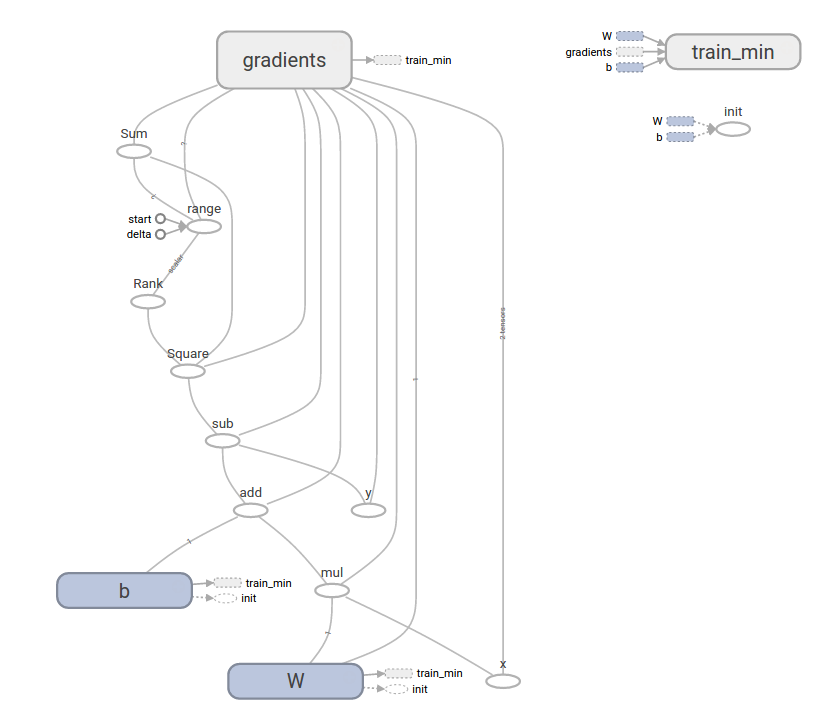
\includegraphics[scale=0.5]{getting_started_final.png}
\caption{整体代码框图}
\end{figure}
\subsubsection{tf.estimators}
tf.estimator是一个改进得TensorFlow库用来简化机器学习机制,包括下面:
\begin{itemize}
\item 运行训练循环
\item 运行估计循环
\item 管理数据集
\end{itemize}
tf.estimators定义了一些常见的模型
\subsubsection{基础用法}
使用tf.estimator线性回归程序变得更简单:
\begin{pythoncode}
# NumPy is often used to load, manipulate and preprocess data.
import numpy as np
import tensorflow as tf

# Declare list of features. We only have one numeric feature. There are many
# other types of columns that are more complicated and useful.
feature_columns = [tf.feature_column.numeric_column("x", shape=[1])]

# An estimator is the front end to invoke training (fitting) and evaluation
# (inference). There are many predefined types like linear regression,
# linear classification, and many neural network classifiers and regressors.
# The following code provides an estimator that does linear regression.
estimator = tf.estimator.LinearRegressor(feature_columns=feature_columns)

# TensorFlow provides many helper methods to read and set up data sets.
# Here we use two data sets: one for training and one for evaluation
# We have to tell the function how many batches
# of data (num_epochs) we want and how big each batch should be.
x_train = np.array([1., 2., 3., 4.])
y_train = np.array([0., -1., -2., -3.])
x_eval = np.array([2., 5., 8., 1.])
y_eval = np.array([-1.01, -4.1, -7, 0.])
input_fn = tf.estimator.inputs.numpy_input_fn(
    {"x": x_train}, y_train, batch_size=4, num_epochs=None, shuffle=True)
train_input_fn = tf.estimator.inputs.numpy_input_fn(
    {"x": x_train}, y_train, batch_size=4, num_epochs=1000, shuffle=False)
eval_input_fn = tf.estimator.inputs.numpy_input_fn(
    {"x": x_eval}, y_eval, batch_size=4, num_epochs=1000, shuffle=False)

# We can invoke 1000 training steps by invoking the  method and passing the
# training data set.
estimator.train(input_fn=input_fn, steps=1000)

# Here we evaluate how well our model did.
train_metrics = estimator.evaluate(input_fn=train_input_fn)
eval_metrics = estimator.evaluate(input_fn=eval_input_fn)
print("train metrics: %r"% train_metrics)
print("eval metrics: %r"% eval_metrics)
\end{pythoncode}
当运行的时候,输出像下面:
\begin{pythoncode}
train metrics: {'average_loss': 1.4833182e-08, 'global_step': 1000, 'loss': 5.9332727e-08}
eval metrics: {'average_loss': 0.0025353201, 'global_step': 1000, 'loss': 0.01014128}
\end{pythoncode}
注意我们的评估数据有一个更高的loss,但是仍然接近于0,这意味了我们正在适当的学习。
\subsubsection{一个自定义的模型}
tf.estimator不限制你使用预先定义的模型。假设我们想创建一个TensorFlow不支持的自定义模型,我们仍然保留数据集的高级抽象,feeding,训练的等等。为了说明这个问题,我们将显示用我们低级API如何实现我们自己的模型LinearRegressor。

为了结合tf.estimator定义自定义的模型,我们需要使用tf.estimator.Estimator。tf.estimator.LinearRegressor实际上是tf.estimator.Estimator的子类。相比于Estimator子类,我们简单提供Estimator一个model\_fn函数高数tf.estimator如何评估预测,训练步数和损失。代码如下:
\begin{pythoncode}
import numpy as np
import tensorflow as tf

# Declare list of features, we only have one real-valued feature
def model_fn(features, labels, mode):
  # Build a linear model and predict values
  W = tf.get_variable("W", [1], dtype=tf.float64)
  b = tf.get_variable("b", [1], dtype=tf.float64)
  y = W*features['x'] + b
  # Loss sub-graph
  loss = tf.reduce_sum(tf.square(y - labels))
  # Training sub-graph
  global_step = tf.train.get_global_step()
  optimizer = tf.train.GradientDescentOptimizer(0.01)
  train = tf.group(optimizer.minimize(loss),
                   tf.assign_add(global_step, 1))
  # EstimatorSpec connects subgraphs we built to the
  # appropriate functionality.
  return tf.estimator.EstimatorSpec(
      mode=mode,
      predictions=y,
      loss=loss,
      train_op=train)

estimator = tf.estimator.Estimator(model_fn=model_fn)
# define our data sets
x_train = np.array([1., 2., 3., 4.])
y_train = np.array([0., -1., -2., -3.])
x_eval = np.array([2., 5., 8., 1.])
y_eval = np.array([-1.01, -4.1, -7., 0.])
input_fn = tf.estimator.inputs.numpy_input_fn(
    {"x": x_train}, y_train, batch_size=4, num_epochs=None, shuffle=True)
train_input_fn = tf.estimator.inputs.numpy_input_fn(
    {"x": x_train}, y_train, batch_size=4, num_epochs=1000, shuffle=False)
eval_input_fn = tf.estimator.inputs.numpy_input_fn(
    {"x": x_eval}, y_eval, batch_size=4, num_epochs=1000, shuffle=False)

# train
estimator.train(input_fn=input_fn, steps=1000)
# Here we evaluate how well our model did.
train_metrics = estimator.evaluate(input_fn=train_input_fn)
eval_metrics = estimator.evaluate(input_fn=eval_input_fn)
print("train metrics: %r"% train_metrics)
print("eval metrics: %r"% eval_metrics)
\end{pythoncode}
当运行时,产生如下:
\begin{pythoncode}
train metrics: {'loss': 1.227995e-11, 'global_step': 1000}
eval metrics: {'loss': 0.01010036, 'global_step': 1000}
\end{pythoncode}
注意自定义的model\_fn()函数的内容类似我们使用低级API训练手动训练模型。








